\documentclass[10pt,a4paper]{article}
\usepackage[utf8]{inputenc}
\usepackage[T1]{fontenc}
\usepackage[spanish,es-noshorthands,es-nodecimaldot,es-tabla]{babel}
\usepackage{amsmath,amssymb}
\usepackage{booktabs,tabularx,array}
\usepackage{graphicx}
\usepackage[margin=1.9cm]{geometry}
\usepackage{enumitem}
\usepackage[font=small,labelfont=bf]{caption}
\usepackage{xcolor}
\usepackage{url}
\def\UrlBreaks{\do\/\do\_}
\newcommand{\dir}[1]{{\scriptsize(\path{#1})}}
\usepackage[colorlinks=true,linkcolor=blue!60!black,urlcolor=blue!60!black]{hyperref}
\graphicspath{{../work/exclusion_comparison/}{../mycodes/}}
\setlist{nosep,leftmargin=1.2em}
\newcommand{\Ap}{A'}
\newcommand{\eps}{\epsilon}
\newcommand{\dd}{\mathrm{d}}
\newcommand{\ttt}[1]{\texttt{\small #1}}
\newcolumntype{L}{>{\raggedright\arraybackslash}X}
\title{\vspace{-1.2cm}Límite de TEXONO sobre fotones oscuros de reactor\\[2pt]
\large Qué hicieron solos los agentes LLM y qué se hizo sobre código humano}
\author{E.~L.~De Paoli\\[2pt]\small escrito con asistencia de agentes (Claude Opus 5.5)}
\date{28 de septiembre de 2026}

\begin{document}
\maketitle
\vspace{-0.6cm}

\section{Objetivo y contexto}
El objetivo era el límite superior al 95\% CL, $\eps_{95}(m_{\Ap})$, sobre la mezcla cinética de un fotón oculto a partir
de los datos de TEXONO (2.9~GW, 28~m, 187~kg de CsI, 160~d, ventana 3--8~MeV), para $m_{\Ap}<1$~MeV. Park (2017) da
$\eps<2.1\times10^{-5}$. Danilov, Demidov y Gorbunov (2019) lo revisan con oscilaciones $\gamma\leftrightarrow\Ap$ en el
medio y con una eficiencia anti-Compton que Park no incluyó. El trabajo está en dos directorios:
\ttt{Proyecto\_Final\_DarkPhoton\_gpt} (Codex) y \ttt{Proyecto\_Final\_DarkPhoton\_claudia} (Claude Code, más las macros
ROOT humanas en \ttt{mycodes/}). Los dos agentes trabajaron con el mismo acuerdo (\ttt{AGENTS.md}): aserciones en vez de
afirmaciones, recibos de ejecución, un \emph{vault} de notas y un \emph{hook} de procedencia que no deja cerrar la sesión
hasta que cada número y cada figura tienen registro.

Todos los enfoques calculan la misma cadena. La producción (ec.~1 de Park) pliega el espectro de fotones del reactor
$S_\gamma$ con la fracción Compton-like; la detección (ec.~7 de Park) cuenta absorciones $\Ap e\to\gamma e$ en la ventana:
\begin{gather}
\frac{\dd N_{\Ap}}{\dd E'}=\int \dd E\,S_\gamma(E)\,\frac{1}{\sigma_{\rm tot}(E)}\frac{\dd\sigma_{\gamma e\to\Ap e}}{\dd E'},\qquad
N_{\rm obs}=\frac{T N_e}{4\pi R^2}\int_{3\,\rm MeV}^{8\,\rm MeV}\!\dd E'\,\frac{\dd N_{\Ap}}{\dd E'}\,\sigma_{\rm abs}(E'),\nonumber\\
\eps_{95}=\eps_{\rm ref}\Big(\frac{N_{95}}{N_{\rm obs}(\eps_{\rm ref})}\Big)^{1/4},
\end{gather}
porque $N_{\rm obs}\propto\eps^4$, con $N_{95}=1.96\times100.6$. Las correcciones tipo Danilov son:
(A) quitar el $2/3$ de Park en $\sigma_{\rm abs}$ (el haz del reactor es transversal);
(B) una eficiencia anti-Compton $\eta=1/6$, es decir $N_{95}\to6N_{95}$;
(D) supresión en el medio $P\propto m_{\Ap}^4/(m_{\Ap}^2-m_\gamma^2)^2$ con $m_\gamma\simeq20$~eV, en producción y en detección;
y, en los modelos de medio de Codex, la oscilación reemplaza a la fuente Compton-like.

\section{Vía 1: trabajo hecho enteramente por agentes LLM}
Estas tareas arrancaron de un \emph{prompt}, del artículo de Park y de artículos que los propios agentes descargaron. No se
usó código humano. Todo es de Codex (OpenAI) salvo la exportación de \emph{skills} (Tabla~\ref{tab:track1}).

\begin{table}[t]
\small
\begin{tabularx}{\textwidth}{@{}>{\raggedright\arraybackslash}p{3.1cm}>{\raggedright\arraybackslash}p{2.3cm}L@{}}
\toprule
Tarea {\scriptsize(directorio)} & Agente & Qué salió \\
\midrule
Bibliografía \dir{dark_photon_papers, papers_reactor_dark_photon} & Codex gpt-5.6-sol, medium; 15--24~min cada una &
36 PDFs con manifiestos y \emph{checksums}, resúmenes HTML bilingües, una \emph{skill} de bibliografía. El corpus de todo lo demás. \\
Reproducción de Park \dir{code/park_texono} & Codex gpt-6-astra, high; 24~min, 6.1\,M tokens &
$\dd\sigma/\dd E'$ exacta a nivel árbol (trazas con SymPy, identidades de Ward, límite Klein--Nishina, chequeo con Gondolo--Raffelt).
Residuos de la Fig.~1 de Park: 4\%, 11\%, 38\% a $m_{\Ap}=0.1,0.5,1$~MeV. $\eps_{95}=1.57\times10^{-5}$; para llegar a 2.1e-5 hace
falta una aceptancia de 0.31, que \emph{no} se aplicó. Escribió Python pese a la regla de usar ROOT, y lo admitió. \\
Solo producción \dir{code/park_production_v2} & Codex, high; 47~min, 5.2\,M tokens &
Todo en C++/ROOT. La sección eficaz coincide con la Ref.~15 a $7\times10^{-14}$; confirma los residuos de la Fig.~1; sin límite. \\
Oscilaciones en el medio \dir{code/darkphoton_v3} & Codex (GPT-6) &
Ecs.~(5), (6), (9) de Danilov frente a la convención de Park; encontró y corrigió un error de coeficiente (4 en vez de 2).
Meseta en el medio $1.335\times10^{-5}$. Digitalizó la curva de TEXONO de Danilov (el único límite publicado digitalizado del proyecto). \\
Decaimiento + barrido sub-MeV \dir{work/reactor_sensitivity} & Codex (GPT-6) &
Agrega el $\Gamma_{3\gamma}$ de Park; irrelevante (profundidad óptica $\le10^{-11}$). Curva de vacío con $\eta=1/6$: $2.45\times10^{-5}$. \\
Desde cero, con Danilov como guía \dir{work/danilov_fresh} & Codex (GPT-6); 49~min &
Producción por oscilación, polarización transversal, decaimiento Euler--Heisenberg con realce de lazo, $\eta=1/6$.
Meseta $1.336\times10^{-5}$ (igual a v3 al 0.1\%); su propio chequeo imprime ``published normalization comparison: FAIL''. \\
Digitalización de la Fig.~1 de Park \dir{work/park_figure1_digitization} & Codex &
Extracción de las tres curvas desde los trazos vectoriales del PDF; luego usada en \ttt{mycodes/}. \\
Exportación de \emph{skills} \dir{skillsforexport} & Claude Opus 5 & La \emph{skill} y el \emph{hook} de procedencia con los que después trabajaron ambos agentes. \\
\bottomrule
\end{tabularx}
\caption{Vía 1: tareas que un agente LLM ejecutó a partir de un \emph{prompt}, sin código humano.}
\label{tab:track1}
\end{table}

\medskip
Codex nunca reprodujo el número de Park, y lo dijo cada vez. Sus límites desde cero caen en dos familias: vacío
Compton-like ($1.57\times10^{-5}$ con $\eta=1$, $2.45\times10^{-5}$ con $\eta=1/6$) y oscilación en el medio
($1.34\times10^{-5}$, $\eta=1/6$).

\section{Vía 2: código e insumos humanos, mejorados con agentes LLM}
\textbf{Insumos humanos.} Una derivación en castellano de la sección eficaz Compton-like (\ttt{apuntes/}, notas de
terceros, no editadas). Además, las macros ROOT de la usuaria \ttt{DP.C}$\to$\ttt{DP2.C}$\to$\ttt{DP3\_Danilov.C}
(E.~L.~De Paoli; se omite el nombre del coautor), que implementan esa derivación: las tablas NIST del uranio, el flujo de fotones FRJ-1 de
Park, las configuraciones de TEXONO y Skipper-CCD, y los interruptores A, B, D. El encabezado de la macro ya acredita
cálculos previos de Claude.

\textbf{Qué hicieron los agentes sobre eso.}
\begin{enumerate}
\item \emph{Auditoría del apunte} (Claude, \ttt{reports/report\_cross\_section\_*.pdf}). Se rederivó la amplitud al
cuadrado exacta con matrices de Dirac explícitas (coincide con la bibliografía a $2\times10^{-13}$). La ec.~(40) del
apunte se desvía entre $-39\%$ y $+33\%$ (pierde los términos en $m_e^2$). Su cinemática usa $|k'|\simeq\omega'$, que pierde
el umbral $E_{\rm th}=m_{\Ap}+m_{\Ap}^2/2m_e$ y el rango verdadero. La ec.~(50) tiene un polo en $\omega'=m_{\Ap}^2/2m_e$ y
sobreestima la tasa en 3--8~MeV en 1.05, 1.46 y 1.99 para $m_{\Ap}=0.1,0.5,1$~MeV. Dos resultados más: el $2/3$ de Park debería ser
$\simeq1$, y el canal de oscilación da $7.7$ veces más $\Ap$ en la ventana que el Compton-like.
\item \emph{Dos errores de normalización en la macro} (Claude). Se usaba $hc$ en vez de $\hbar c$ ($\sigma$ 39.5 veces
grande), y la sección eficaz NIST es por átomo, no por electrón (92 veces chica, $Z_U=92$). Se compensan hasta un factor
2.33: por eso la macro original parecía coincidir con Park. La usuaria aplicó ambas correcciones (22/09) y pasó la
cinemática exacta a \ttt{DP3\_Danilov.C} (23/09), pero mantuvo la ec.~(50).
\item \emph{\ttt{DP3\_Danilov\_new.C}} (Claude). Una copia con funciones \ttt{*\_new\_f}: la sección eficaz exacta y el
rango de fotones exacto \ttt{Rw\_new\_f} ($x_-(\omega)$ no es monótona, así que se busca numéricamente). Las funciones
originales quedan intactas.
\item \emph{Comparación de la Fig.~1} (Codex, \ttt{mycodes/combined\_figure1.C}). Los espectros de la macro sobre la
digitalización de Park hecha por Codex (Fig.~\ref{fig:fig1}).
\item \emph{Este informe} (Claude). Extrae la curva de TEXONO de ambas macros con los interruptores apagados y encendidos,
sin editarlas (\ttt{work/exclusion\_comparison/}), y prueba la grilla en $E_{\Ap}$.
\end{enumerate}

\begin{figure}[t]
\centering
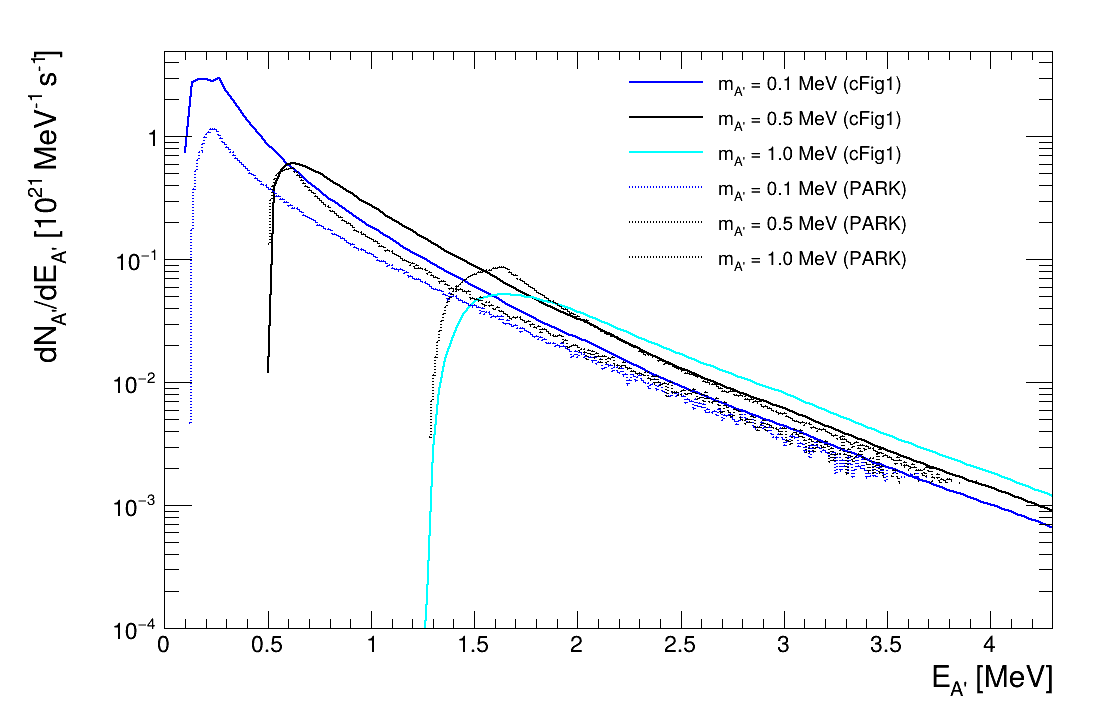
\includegraphics[width=0.52\textwidth]{combined_figure1.png}
\caption{Fig.~1 de Park ($\dd N_{\Ap}/\dd E_{\Ap}$ a 1~GW, $\eps=1$): \ttt{DP3\_Danilov.C} actual (continua) frente a la
digitalización del artículo hecha por Codex (punteada). \ttt{mycodes/combined\_figure1.C}. Formas y umbrales coinciden; la
curva de 0.1~MeV queda $\sim$2.5 veces más alta en el pico. La cola de Park por encima de 2~MeV sigue al propio espectro de
fotones, no a su ec.~(1) (auditoría de Claude, \S7), así que esta figura no sirve para ajustar la normalización.}
\label{fig:fig1}
\end{figure}

\section{Todos los límites de exclusión en un gráfico}
La Figura~\ref{fig:excl} pone todos los enfoques sobre los mismos ejes. El color indica quién escribió el código: negro =
publicado, azul = macro humana, naranja = macro humana con la sección eficaz exacta de Claude, verde/violeta/magenta = Codex
desde cero. El tipo de línea indica la física: continua = vacío/estilo Park, a trazos = correcciones tipo Danilov. La
Tabla~\ref{tab:eps} da los valores.

\begin{figure}[p]
\centering
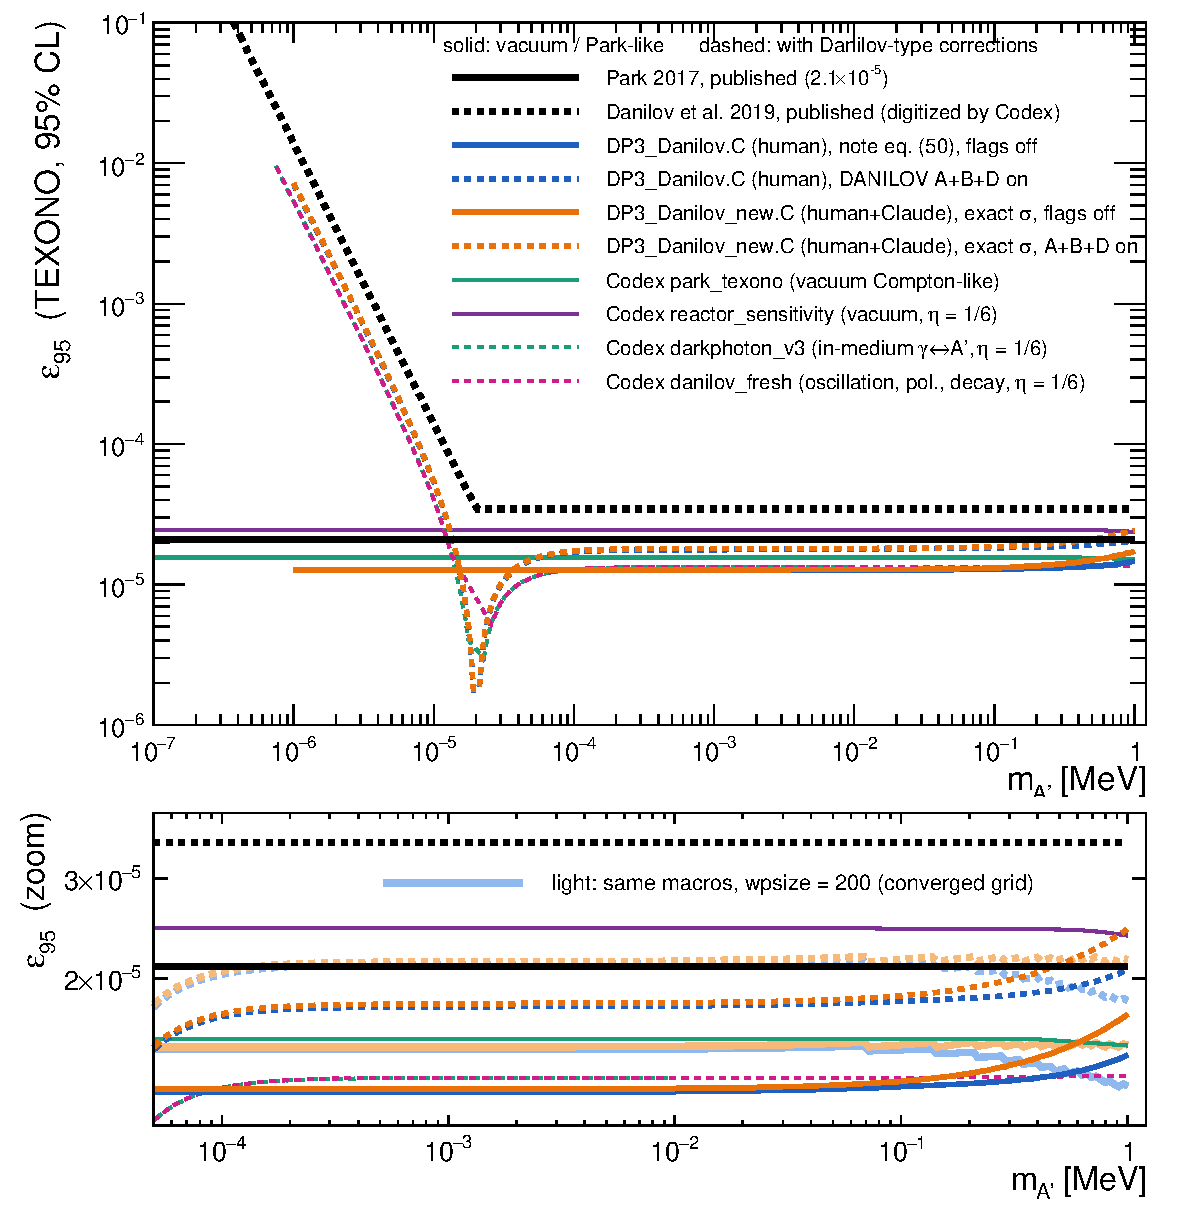
\includegraphics[width=0.97\textwidth]{texono_exclusion_all.pdf}
\caption{$\eps_{95}$ de TEXONO en función de $m_{\Ap}$. Las curvas de las macros humanas se extraen del canvas \ttt{cSk} de
\ttt{DP3\_Danilov.C} y \ttt{DP3\_Danilov\_new.C}, con su grilla por defecto (\ttt{wpsize}\,=\,10); el zoom agrega las
mismas corridas con \ttt{wpsize}\,=\,200 (colores claros). Las curvas de Codex se leen tal cual de sus CSV (se saltean las
filas nan). Park: el valor citado $2.1\times10^{-5}$. Danilov: la digitalización de Codex, plana por encima de 20.6~eV. Abajo:
zoom sobre la meseta. Leyendas en inglés, como en las macros. Generado por \ttt{work/exclusion\_comparison/run.sh}.}
\label{fig:excl}
\end{figure}

\begin{table}[t]
\centering\small\setlength{\tabcolsep}{4.5pt}
\begin{tabular}{@{}lllcccccc@{}}
\toprule
Curva & de & física & $10^{-6}$ & $10^{-4}$ & $10^{-2}$ & 0.1 & 0.5 & 1.0~MeV\\
\midrule
Park 2017 & publicado & vacío, $2/3$, $\eta=1$ & 2.10 & 2.10 & 2.10 & 2.10 & 2.10 & 2.10\\
Danilov 2019 & publicado & medio, $\eta=1/6$ & 1264 & 3.47 & 3.47 & 3.47 & 3.47 & 3.47\\
\ttt{DP3\_Danilov.C}, off & humano & ec.~(50), vacío & 1.26 & 1.26 & 1.26 & 1.29 & 1.35 & 1.47\\
\ttt{DP3\_Danilov.C}, A+B+D & humano & ec.~(50) + A, B, D & 711 & 1.71 & 1.79 & 1.82 & 1.91 & 2.07\\
\ttt{\_new.C} exacta, off & humano+Claude & $\sigma$ exacta, vacío & 1.28 & 1.28 & 1.28 & 1.32 & 1.49 & 1.73\\
\ttt{\_new.C} exacta, A+B+D & humano+Claude & $\sigma$ exacta + A, B, D & 720 & 1.73 & 1.81 & 1.86 & 2.11 & 2.44\\
\multicolumn{9}{@{}l}{\emph{las mismas dos macros, grilla convergida (\ttt{wpsize}\,=\,200):}}\\
\ttt{DP3\_Danilov.C}, off & humano & ec.~(50), vacío & 1.50 & 1.50 & 1.50 & 1.50 & 1.38 & 1.29\\
\ttt{DP3\_Danilov.C}, A+B+D & humano & ec.~(50) + A, B, D & 844 & 2.03 & 2.12 & 2.11 & 1.95 & 1.83\\
\ttt{\_new.C} exacta, off & humano+Claude & $\sigma$ exacta, vacío & 1.51 & 1.51 & 1.52 & 1.53 & 1.52 & 1.53\\
\ttt{\_new.C} exacta, A+B+D & humano+Claude & $\sigma$ exacta + A, B, D & 854 & 2.06 & 2.15 & 2.16 & 2.16 & 2.16\\
\midrule
\ttt{park\_texono} & Codex & vacío, $2/3$, $\eta=1$ & 1.57 & 1.57 & 1.57 & 1.57 & 1.56 & 1.52\\
\ttt{reactor\_sensitivity} & Codex & vacío, $\eta=1/6$ & 2.45 & 2.45 & 2.45 & 2.45 & 2.44 & 2.38\\
\ttt{darkphoton\_v3} & Codex & oscilación, $\eta=1/6$ & 518 & 1.28 & 1.34 & -- & -- & --\\
\ttt{danilov\_fresh} & Codex & oscilación + pol.\ + decaim. & 533 & 1.28 & 1.34 & 1.34 & 1.34 & 1.34\\
\bottomrule
\end{tabular}
\caption{$\eps_{95}$ en unidades de $10^{-5}$ en el punto de grilla más cercano a cada masa (``--'': no hay punto, o está
fuera de la validez declarada del modelo; v3 termina en 10~keV). Impreso por \ttt{exclusion\_comparison.C::table\_row}.}
\label{tab:eps}
\end{table}

\textbf{Qué dice el gráfico.}
\begin{enumerate}
\item \emph{En la meseta todos los enfoques caen dentro de un factor 2 de Park}, entre $1.26$ y $2.45\times10^{-5}$.
Ningún enfoque, humano o LLM, reproduce $2.1\times10^{-5}$ con los insumos del propio Park. Para el cálculo de vacío estilo
Park, la macro humana da 1.26 y Codex 1.57 (en $10^{-5}$).
\item \emph{La meseta de la macro humana no está convergida en la grilla de $E_{\Ap}$.} Con \ttt{wpsize}\,=\,10 caen
solo $\sim$5 puntos en la ventana de 3--8~MeV. Al subirlo, la meseta con interruptores apagados pasa de 1.26 a 1.50
(\ttt{wpsize}\,=\,200; con 400 cambia otro 0.5\%). La subida hacia 1~MeV de las curvas por defecto es ruido de grilla:
convergida, la ec.~(50) \emph{baja} a 1.29 en 1~MeV. Con la sección eficaz exacta de Claude y la grilla convergida, la macro
da 1.51 en la meseta y 1.525 en 1~MeV. El \ttt{park\_texono} de Codex, independiente, da 1.57 y 1.52. \textbf{El código
humano con la sección eficaz corregida y el código escrito desde cero por otro LLM coinciden al 3\% en la meseta y al
0.3\% en 1~MeV.} Es el único chequeo cruzado real entre las dos vías.
\item \emph{Sección eficaz exacta frente a la ec.~(50)} (convergida). Despreciable en la meseta (1\%). En 1~MeV la curva
exacta es 18\% más débil (1.525 contra 1.29): es la sobreestimación de 1.99 veces de la tasa con la ec.~(50), elevada a la
$1/4$.
\item \emph{Los límites tipo Danilov no coinciden con el gráfico de Danilov.} Con la grilla por defecto, la macro con
A+B+D da 1.71; convergida, 2.03--2.06. Ese valor está cerca del 2.1 de Park, pero solo porque los factores de A y B se
combinan casualmente hasta ahí. La macro mantiene la fuente Compton-like y la multiplica por la supresión. Los modelos de
oscilación de Codex dan 1.34, y la curva publicada de Danilov, 3.47. El número de Park reescalado solo por B,
$2.1\times6^{1/4}=3.29$, queda a 5\% de la meseta de Danilov. Por encima de $m_\gamma$, entonces, la curva de Danilov es
compatible con el resultado de Park multiplicado por la eficiencia. Es una observación numérica, no algo que diga el
artículo.
\item \emph{Por debajo de $m_\gamma\simeq20$~eV} todas las curvas tipo Danilov suben como $\eps\propto m_{\Ap}^{-2}$, porque
$N_{\rm obs}\propto(m/m_\gamma)^8$. En 1~eV todas quedan entre 1.5 y 2.4 veces por debajo de la de Danilov. El pozo profundo de
la curva humana en 19.2~eV ($1.8\times10^{-6}$) es un artefacto: \ttt{danilov\_suppression} se corta en 100 en vez de
conservar el ancho de la resonancia. Codex saca una ventana alrededor de la resonancia (filas nan), así que sus curvas
muestran un pozo menos profundo.
\end{enumerate}

\section{Balance}
\begin{itemize}
\item \textbf{Coincidencias.} Los dos agentes derivaron por separado la sección eficaz exacta de $\gamma e\to\Ap e$ y la
verificaron a $10^{-13}$. Ninguna de las dos vías reproduce la normalización de Park con sus insumos declarados.
\item \textbf{LLM solo.} Rápido y bien documentado: recibos, procedencia, informes bilingües. Pero produjo cuatro límites
desde cero repartidos en un factor 1.8, ninguno igual a una curva publicada. Cuando no reprodujo el objetivo, lo dijo en vez
de ajustar. Una vez rompió las reglas del \emph{prompt} de Codex (solo ROOT).
\item \textbf{Código humano + LLM.} Acá se encontraron y corrigieron los errores: el polo y la cinemática del apunte, los
errores de normalización $hc/\hbar c$ y por átomo que se tapaban entre sí, y ahora el \ttt{wpsize} grueso. Con todos
corregidos, la cadena humana cae sobre el número de Codex. La macro humana lleva el conocimiento del experimento
(proyecciones Skipper-CCD, los interruptores de Danilov) que ningún agente escribió.
\item \textbf{Pendiente.} Nadie reproduce el $2.1\times10^{-5}$ de Park. La normalización tipo Danilov no está resuelta
(factor 2.6 entre Codex y el artículo). \ttt{DP3\_Danilov.C} todavía usa la ec.~(50), \ttt{wpsize}\,=\,10 y la resonancia
cortada (cambiarlos lo decide la usuaria; para este informe no se editó ningún archivo de \ttt{mycodes/}). $m_\gamma$ es un
valor de referencia (20~eV), nunca calculado a partir de los materiales.
\end{itemize}

\noindent\textit{No verificado acá}: los CSV y la digitalización de Codex se leyeron tal cual; los códigos de Codex no se
volvieron a correr. Modelo, esfuerzo y tokens de las dos tareas de Park salen de los registros de sesión de Codex; los demás
informes dicen ``not exposed'', y también el informe de auditoría de Claude.

\end{document}
